% Adjust these for the path of the theme and its graphics, relative to this file
%\usepackage{beamerthemeFalmouthGamesAcademy}
\usepackage{../../beamerthemeFalmouthGamesAcademy}
\usepackage{multimedia}
\graphicspath{ {../../} }

% Default language for code listings
\lstset{language=C++,
        morekeywords={each,in,nullptr}
}

% For strikethrough effect
\usepackage[normalem]{ulem}
\usepackage{wasysym}

\usepackage{pdfpages}

\begin{document}
\title{Software Testing}   
\subtitle{COMP110: Principles of Computing}

\frame{\titlepage} 

% Testing
% C++
%   Composition
%   Ownership
% Finite state machines
% COMP110 coding task 2

\begin{frame}{Today's lecture}
    Today's lecture has \textbf{three parts}
    \begin{itemize}
        \item Software testing and test-driven development
        \item Introducing COMP110 Coding Task II
        \item Object composition in C++
    \end{itemize}
\end{frame}

\part{Software testing}
\frame{\partpage}

\begin{frame}{In this section}
    In this section you will learn how to:
    \begin{itemize}
        \item \textbf{Discuss} the importance of software testing in game development
        \item \textbf{Identify} the different types and levels of testing
        \item \textbf{Apply} test-driven development practices to your own programming projects
    \end{itemize}
\end{frame}

\begin{frame}{Further reading}
    \begin{itemize}
        \item Pressman, R.S. (2009) Software Engineering: A Practitioner's Approach. 7th Edition. McGraw-Hill.
    \end{itemize}
\end{frame}

\begin{frame}{Quality}
    Last time: \pause
    \begin{itemize}
        \item There are many ways of measuring the \textbf{quality} of a game or piece of software \pause
        \item \textbf{Quality assurance} is important to ensure that the software is of sufficiently high
            quality to provide benefit to developers and end users
    \end{itemize}
\end{frame}

\begin{frame}{Testing}
    \begin{itemize}
        \item Finding \textbf{inadvertent errors} in the design and implementation of software \pause
        \item Often takes more time and effort than any other part of development \pause
        \item ... but letting errors slip into the final product can be even more costly \pause
        \item Testing $\neq$ quality assurance \pause
            \begin{itemize}
                \item Testing is an important part of QA, but \textbf{not the only part}
            \end{itemize}
    \end{itemize}
\end{frame}

\begin{frame}{Who is responsible?}
    \begin{itemize}
        \item Last time, we discussed that \textbf{designers}, \textbf{developers},
            \textbf{publishers}, and maybe even \textbf{players}
            share the responsibility for software quality in games \pause
        \item Who should take responsibility for \textbf{testing}? \pause
            \begin{itemize}
                \item ``\textbf{Developers} write the code, so they should make sure it works''? \pause
                \item ``\textbf{Everyone} is responsible for quality, so everyone should pitch in''? \pause
                \item ``Code should be tested by \textbf{someone other} than the developer who wrote it''?
            \end{itemize}
    \end{itemize}
\end{frame}

\begin{frame}{Socrative \texttt{6E8NSW3IN}}
    So who should test game software?
	\begin{itemize}
		\item In pairs.
		\item Discuss for 2-minutes.
		\item \textbf{Suggest} which parties should take responsibility for testing \textbf{and justify} your answer. 
	\end{itemize}
\end{frame}

\begin{frame}{Testing strategy}
    \begin{center}
        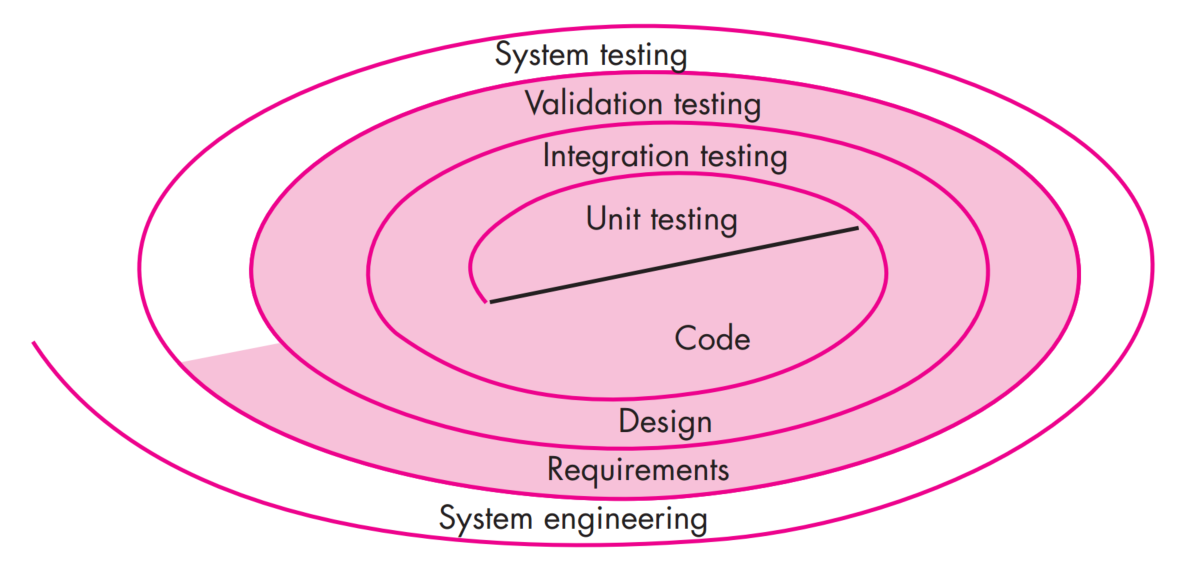
\includegraphics[width=\textwidth]{pressman_17_1}
        
        {\tiny [Pressman, 2009] Figure 17.1}
    \end{center}
\end{frame}

\begin{frame}{Testing strategy}
    \begin{itemize}
        \item Development starts with system engineering and works \textbf{inwards} \pause
            \begin{itemize}
                \item The \textbf{waterfall model} \pause
                \item Agile doesn't quite work like this \pause
            \end{itemize}
        \item Testing starts with unit testing and works \textbf{outwards} \pause
        \item \textbf{White box testing}: testing the software \textbf{with} knowledge of its internal workings \pause
        \item \textbf{Black box testing}: testing the software \textbf{without} knowledge of its internal workings
    \end{itemize}
\end{frame}

\begin{frame}{Unit testing}
    \begin{itemize}
        \item A \textbf{unit test} is a piece of code that verifies a \textbf{unit} (e.g.\ a function or class) of a program \pause
        \item E.g.\ verifies that a function called with a particular set of parameters returns the expected result \pause
        \item E.g.\ verifies that a function called with invalid parameters throws the expected error
    \end{itemize}
\end{frame}

\begin{frame}{Designing unit tests}
    \begin{itemize}
        \item Test the \textbf{edge cases} \pause
            \begin{itemize}
                \item Programming errors often occur at the \textbf{boundary} between valid and invalid input,
                    or the boundary between one case and another \pause
                \item E.g.\ for an $n$-element data structure, test accessing elements $n-1$, $n$, $n+1$ \pause
            \end{itemize}
        \item Aim for high \textbf{coverage} \pause
            \begin{itemize}
                \item Ideally, \textbf{every line of code} should be executed in \textbf{at least one} unit test
            \end{itemize}
    \end{itemize}
\end{frame}

\begin{frame}{Drivers and stubs}
    \begin{columns}
        \begin{column}{0.48\textwidth}
            \begin{center}
                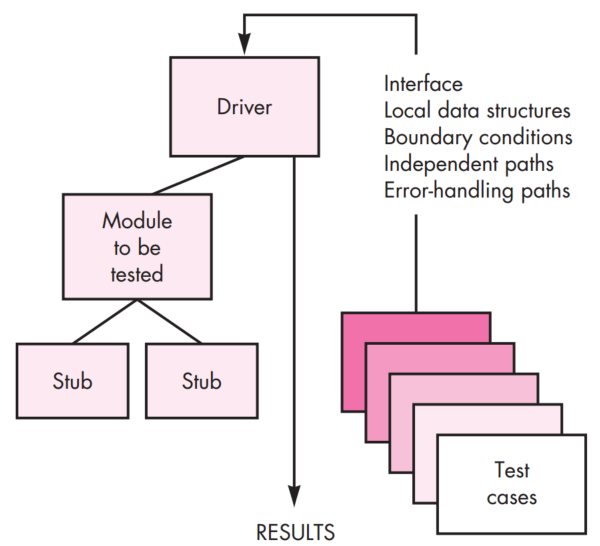
\includegraphics[width=\textwidth]{pressman_17_4}
                
                {\tiny [Pressman, 2009] Figure 17.4}
            \end{center}
        \end{column}
        \begin{column}{0.48\textwidth}
            \begin{itemize}
                \item Unit testing generally requires extra code to be written \pause
                \item \textbf{Driver} --- to set up any required state and run the test \pause
                \item \textbf{Stubs} --- to replace any modules upon which the module under test depends
            \end{itemize}
        \end{column}
    \end{columns}
\end{frame}

\begin{frame}{Integration testing}
    \begin{itemize}
        \item Verify that the individual units work \textbf{together} \pause
        \item Can be done \textbf{top-down} or \textbf{bottom-up} \pause
        \item Either way, the idea is to gradually replace stubs and drivers with actual units,
            testing as you go \pause
        \item \textbf{Regression testing} is important --- re-running tests to ensure that recent additions
            have not broken anything
    \end{itemize}
\end{frame}

\begin{frame}{Socrative \texttt{6E8NSW3IN}}
	If the units have been thoroughly tested individually, why is integration testing needed?
	\begin{itemize}
		\item In pairs.
		\item Discuss for 2-minutes.
		\item Give an \textbf{example} of a problem that integration testing might uncover,
            but that unit testing might miss. 
	\end{itemize}
\end{frame}

\begin{frame}{Validation testing}
    \begin{itemize}
        \item Testing the complete software system from the user's point of view \pause
        \item E.g.\ playtesting
    \end{itemize}
\end{frame}

\begin{frame}{Socrative \texttt{6E8NSW3IN}}
	If unit testing and integration testing have been done correctly, why is validation testing needed?
	\begin{itemize}
		\item In pairs.
		\item Discuss for 2-minutes.
		\item Give an \textbf{example} of a problem that validation testing might uncover,
            but that unit and integration testing might miss. 
	\end{itemize}
\end{frame}

\begin{frame}{When is testing ``done''?}
    \begin{itemize}
        \item The aim of testing is to find bugs, so it's done when there are no bugs left to be found! \smiley{} \pause
        \item When the software is (quantitatively or qualitatively) ``good enough'' \pause
        \item Testing is never ``done'' --- the burden just shifts onto the users
    \end{itemize}
\end{frame}

\begin{frame}{Test driven development (TDD)}
    \begin{itemize}
        \item A development process that advocates writing the unit tests \textbf{first} \pause
        \item Repeat the following three steps: \pause
            \begin{enumerate}
                \item \textbf{Red}: create a new test case, which should initially \textbf{fail} \pause
                \item \textbf{Green}: write code to make the new test \textbf{succeed} (without causing the other test cases to fail) \pause
                \item \textbf{Refactor}: \textbf{improve} the code, ensuring that all tests still \textbf{succeed}
            \end{enumerate}
    \end{itemize}
\end{frame}

\begin{frame}{Why TDD?}
    \begin{itemize}
        \item Often easier to convert a \textbf{user story} into test cases rather than directly into code \pause
        \item Writing the bare minimum of code to make the test ``green''
            lets you \textbf{focus on user stories}, not on \textbf{over-generalisation} or \textbf{non-essential functionality} \pause
            \begin{itemize}
                \item \textbf{KISS}: Keep It Simple, Stupid
                \item \textbf{YAGNI}: You Aren't Gonna Need It
            \end{itemize}
    \end{itemize}
\end{frame}

\begin{frame}{Red}
    \begin{itemize}
        \item Create a new test case, which should initially \textbf{fail} \pause
        \item Write only enough code to allow the test case to compile and run,
            e.g.\ write a \textbf{stub} function \pause
        \item What if the test succeeds? \pause
            \begin{itemize}
                \item Maybe you already implemented that feature? \pause
                \item Maybe the test case is wrong? \pause
                \item Maybe your unit testing code is broken?
            \end{itemize}
    \end{itemize}
\end{frame}

\begin{frame}{Green}
    \begin{itemize}
        \item Add the \textbf{bare minimum} of code to make the new test case succeed \pause
            \begin{itemize}
                \item \textbf{K}eep \textbf{I}t \textbf{S}imple, \textbf{S}tupid! \pause
            \end{itemize}
        \item Verify that \textbf{all} unit tests now succeed \pause
        \item What if old tests now fail? \pause
            \begin{itemize}
                \item Fix it \pause
                \item \textbf{Or} revert and start again --- can be faster than debugging \pause
                \item (you \textbf{did} commit before you started, right?)
            \end{itemize}
    \end{itemize}
\end{frame}

\begin{frame}{Refactor}
    \begin{itemize}
        \item E.g. remove duplication, improve names, add documentation, apply design patterns, ... \pause
        \item To generalise or not to generalise? \pause
        \item \textbf{Do} generalise if it makes the code \textbf{simpler} \pause
        \item \textbf{Don't} generalise because you ``might'' need it later \pause
            \begin{itemize}
                \item \textbf{Y}ou \textbf{A}ren't \textbf{G}onna \textbf{N}eed \textbf{I}t!
                \item Wait until it \textbf{is} needed in another cycle \pause
            \end{itemize}
        \item Verify that \textbf{all} unit tests still succeed
    \end{itemize}
\end{frame}

\begin{frame}{Socrative \texttt{6E8NSW3IN}}
	How suitable is the test driven approach for game development?
	\begin{itemize}
		\item In pairs.
		\item Discuss for 2-minutes.
		\item Suggest \textbf{one advantage and one disadvantage} of test driven development
            in the context of game development
	\end{itemize}
\end{frame}

\begin{frame}{Summary}
    \begin{itemize}
        \item \textbf{Testing} is an important part of software quality assurance (but not the only part)
        \item There are several different \textbf{levels} of testing,
            which mirror the different levels of software development
            \begin{itemize}
                \item Unit testing $\leftrightarrow$ Coding
                \item Integration testing $\leftrightarrow$ Design
                \item Validation testing $\leftrightarrow$ Requirement planning
            \end{itemize}
        \item \textbf{Test driven development} is one possible strategy for testing your software
            (but not the only strategy)
    \end{itemize}
\end{frame}

\part{COMP110 Coding Task 2}
\frame{\partpage}

\begin{frame}{The assignment brief}
\begin{center}
    LearningSpace: COMP110 assignment 4
\end{center}
\end{frame}

\begin{frame}{The task}
    \begin{itemize}
        \item Develop a \textbf{component}... \pause
            \begin{itemize}
                \item \textbf{For example}, non-player character AI
                \item \textbf{or} procedural content generator
                \item \textbf{or} physics simulation
                \item \textbf{or} combat mechanic
                \item \textbf{or} ...
            \end{itemize} \pause
        \item ... for a \textbf{game} \pause
            \begin{itemize}
                \item BA Digital Games project
                \item \textbf{or} your COMP150 group project
                \item \textbf{or} your COMP130 Kivy project
            \end{itemize}
    \end{itemize}
\end{frame}

\begin{frame}{How does this fit with COMP150?}
    \begin{itemize}
        \item You will take \textbf{ownership} of this component of the game \pause
            \begin{itemize}
                \item Essentially as a ``consultant'' to your own team
            \end{itemize} \pause
        \item Members of the same COMP150 team \textbf{must not} target the same component of their COMP150 game
    \end{itemize}
\end{frame}

\begin{frame}{Proposal}
    \begin{itemize}
        \item For \textbf{next Wednesday's COMP110 lecture (9th March)}
        \item See assignment brief for details
    \end{itemize}
\end{frame}

\part{Composition in C++}
\frame{\partpage}

\begin{frame}{From COMP110 session 7}
    OOP models three types of relationship: \pause
    \begin{itemize}
        \item \textbf{Is-a}: modelled by \textbf{instantiation} \pause
        \item \textbf{Has-a}: modelled by \textbf{composition} \pause
        \item \textbf{Is-a-type-of}: modelled by \textbf{inheritance}
    \end{itemize}
\end{frame}

\begin{frame}[fragile]{Composition in Python}
    \begin{itemize}
        \item ``A duck has a bill'' $\to$
            ``Each instance of class Duck contains a reference to an instance of class Bill'' \pause
    \end{itemize}
    \begin{lstlisting}[language=Python]
class Bill:
    ...

class Duck:
    def __init__(self):
        self.bill = Bill()
    \end{lstlisting} \pause
    \begin{itemize}
        \item Why a \textbf{reference}? \pause
        \item Because that's your only option in Python!
    \end{itemize}
\end{frame}

\begin{frame}[fragile]{Composition in C++}
    \begin{center}
        ``A duck has a bill''
    \end{center}
    \pause
    \begin{columns}
        \begin{column}{0.48\textwidth}
            \begin{itemize}
                \item ``Each instance of class Duck contains \textbf{an instance} of class Bill''
            \end{itemize}
            \begin{lstlisting}
class Bill { ... };

class Duck
{
private:
    Bill bill;
};
            \end{lstlisting}
        \end{column}
        \pause
        \begin{column}{0.48\textwidth}
            \begin{itemize}
                \item \textbf{Or} ``Each instance of class Duck contains \textbf{a pointer} to an instance of class Bill''
            \end{itemize}
            \begin{lstlisting}
class Bill { ... };

class Duck
{
private:
    Bill* bill;
};
            \end{lstlisting}
        \end{column}
    \end{columns}
\end{frame}

\begin{frame}{Composition in C++}
    \begin{columns}
        \begin{column}{0.55\textwidth}
            \begin{itemize}
                \item The contained instance of \lstinline{Bill} is stored \textbf{inside} the
                    instance of \lstinline{Duck} (literally, in memory) \pause
                \item It is constructed when the \lstinline{Duck} instance is constructed,
                    and destroyed when it is destroyed \pause
            \end{itemize}
        \end{column}
        \begin{column}{0.5\textwidth}
            \begin{itemize}
                \item The contained instance of \lstinline{Bill} is stored \textbf{outside} the
                    instance of \lstinline{Duck}, which only stores a \textbf{pointer} \pause
                \item It is usually constructed manually using \lstinline{new},
                    and so must be destroyed manually using \lstinline{delete}
            \end{itemize}
        \end{column}
    \end{columns}
\end{frame}

\begin{frame}{When to use each?}
    \begin{itemize}
        \item Pointers are more versatile \pause
            \begin{itemize}
                \item Allow several pointers to the same instance (e.g.\ several ducks might \textbf{have-a} single pond) \pause
                \item Allow \textbf{circular references} (e.g.\ a duck \textbf{has-a} bill, and a bill \textbf{has-a} duck) \pause
                \item Pointers allow \textbf{polymorphism} (e.g.\ a pointer to a ``duck'' might actually be a pointer to a mallard) \pause
            \end{itemize}
        \item \textbf{But} stored instances are easier to work with \pause
            \begin{itemize}
                \item Destruction is handled automatically \pause
            \end{itemize}
        \item They model slightly different types of \textbf{has-a} relationship \pause
            \begin{itemize}
                \item Instance: \textbf{has-a} in the sense of ``contains'' \pause
                \item Pointer: \textbf{has-a} in the sense of ``is associated with''
            \end{itemize}
    \end{itemize}
\end{frame}

\begin{frame}[fragile]{Circular references}
    \begin{itemize}
        \item The following code won't compile:
    \end{itemize}
    \begin{lstlisting}
class Bill
{
private:
    Duck* owner;   // Error here
};

class Duck
{
private:
    Bill bill;
};
    \end{lstlisting}
\end{frame}

\begin{frame}[fragile]{What's the problem?}
    \begin{itemize}
        \item \textbf{Order} of definitions and declarations matters in C++ \pause
        \item You \textbf{can't} use something \textbf{before} it's been declared \pause
        \item The offending line is using \lstinline{Duck} before it's declared \pause
        \item Does this make circular referencing impossible?
            Need to declare \lstinline{Duck} before \lstinline{Bill},
            but also need to declare \lstinline{Bill} before \lstinline{Duck} \pause
            \begin{itemize}
                \item No...
            \end{itemize}
    \end{itemize}
\end{frame}

\begin{frame}[fragile]{Forward declarations}
    \begin{itemize}
        \item Solution: use a \textbf{forward declaration} \pause
    \end{itemize}
    \begin{lstlisting}
class Duck;   // Forward declaration

class Bill
{
private:
    Duck* owner;   // This is OK now
};

class Duck
{
private:
    Bill bill;
};
    \end{lstlisting}
\end{frame}

\begin{frame}[fragile]{Socrative \texttt{6E8NSW3IN}}
    \begin{itemize}
        \item Different code, same problem:
    \end{itemize}
    
    \begin{columns}
        \begin{column}{0.4\textwidth}
            Bill.h
            \begin{lstlisting}[numbers=left, numberstyle=\tiny\texttt]
#pragma once

#include "Duck.h"

class Bill
{
private:
    Duck* owner;
};
            \end{lstlisting}
        \end{column}
        \begin{column}{0.4\textwidth}
            Duck.h
            \begin{lstlisting}[numbers=left, numberstyle=\tiny\texttt]
#pragma once

#include "Bill.h"

class Duck
{
private:
    Bill bill;
};
            \end{lstlisting}
        \end{column}
    \end{columns}
    \begin{itemize}
        \item How to fix it?
        \item Discuss \textbf{in pairs} for 2 minutes and post your answer
    \end{itemize}
\end{frame}

\begin{frame}[fragile]{Limitations of forward declarations}
    \begin{itemize}
        \item Basically all you can do with a forward declared class is declare a \textbf{pointer} to it \pause
        \item E.g.\ this wouldn't work:
    \end{itemize}
    \begin{lstlisting}
class Bill;

class Duck
{
private:
    Bill bill; // Error: undefined class 'Bill'
};

class Bill
{
private:
    Duck* owner;
};
    \end{lstlisting}
\end{frame}

\begin{frame}{Limitations of forward declarations}
    \begin{itemize}
        \item The compiler needs to know \textbf{how big} (in bytes) an instance of \lstinline{Bill} is,
            which the forward declaration doesn't tell it \pause
        \item \textbf{All pointers have the same size}, so a forward declaration is enough in that case \pause
        \item Circular references of contained instances are \textbf{impossible} \pause
            \begin{itemize}
                \item At least one of the links in the chain must be a \textbf{pointer} \pause
                \item ``Contains-a'' relationships in real life can't be circular either \pause
                \item Philosophical thought for the day: how big would something have to be,
                    to be big enough to contain itself?
            \end{itemize}
    \end{itemize}
\end{frame}

\begin{frame}[fragile]{Composition and containers}
    \begin{lstlisting}
std::vector<Duck> ducks;
    \end{lstlisting}
    \pause
    \begin{itemize}
        \item The instances are stored \textbf{consecutively} in memory \pause
        \item What happens when the size of the \lstinline{vector} changes? \pause
            \begin{itemize}
                \item \textbf{Recall}: when the size of a \lstinline{vector} changes,
                    a new array is allocated, the contents are \textbf{copied} into it
                    and the old array is \textbf{destroyed} \pause
            \end{itemize}
        \item This can result in unexpected calls to your \textbf{copy constructor}
            and \textbf{destructor} \pause
        \item Can cause problems when using certain idioms (e.g.\ \textbf{RAII})
    \end{itemize}
\end{frame}

\begin{frame}[fragile]{Composition and containers}
    \begin{lstlisting}
std::vector<Duck*> ducks;
    \end{lstlisting}
    \pause
    \begin{itemize}
        \item This is a \lstinline{vector} of \textbf{pointers} \pause
        \item When the \lstinline{vector} changes size,
            the instances stay where they are ---
            only the \textbf{pointers} are copied \pause
        \item \textbf{However}, managing instances with \lstinline{new} and \lstinline{delete}
            is now your responsibility
    \end{itemize}
\end{frame}

\begin{frame}{Ownership}
    \begin{itemize}
        \item It is important to keep track of which module ``\textbf{owns}'' a particular instance \pause
        \item The owner is responsible for \lstinline{delete}ing the instance when it is no longer
            needed \pause
        \item Code should \textbf{never} \lstinline{delete} an instance that it does not own \pause
        \item Generally ownership stays with the module that created the instance,
            \textbf{unless} it explicitly transfers it \pause
            \begin{itemize}
                \item In which case, \textbf{document this clearly} in the module documentation \pause
                \item If you take ownership of a pointer, \lstinline{delete}ing it is now your responsibility \pause
            \end{itemize}            
        \item NB: C++ doesn't care about ownership --- it's a concept \textbf{we} use to write and understand programs
    \end{itemize}
\end{frame}

\begin{frame}{Summary}
    \begin{itemize}
        \item \textbf{Composition} models \textbf{has-a} relationships, which can include
            \textbf{contains-a} and \textbf{is-associated-with-a}
        \item \textbf{Circular references} can be set up using pointers,
            but \textbf{forward declarations} are often needed to make the compiler understand them
        \item \textbf{Ownership} is one way of keeping track of instances and understanding
            when to \lstinline{delete} them
    \end{itemize}
\end{frame}


% -------------------------------------------------------

%\part{The compiler}
%\frame{\partpage}
%
%\begin{frame}
%	\frametitle{The build process}
%	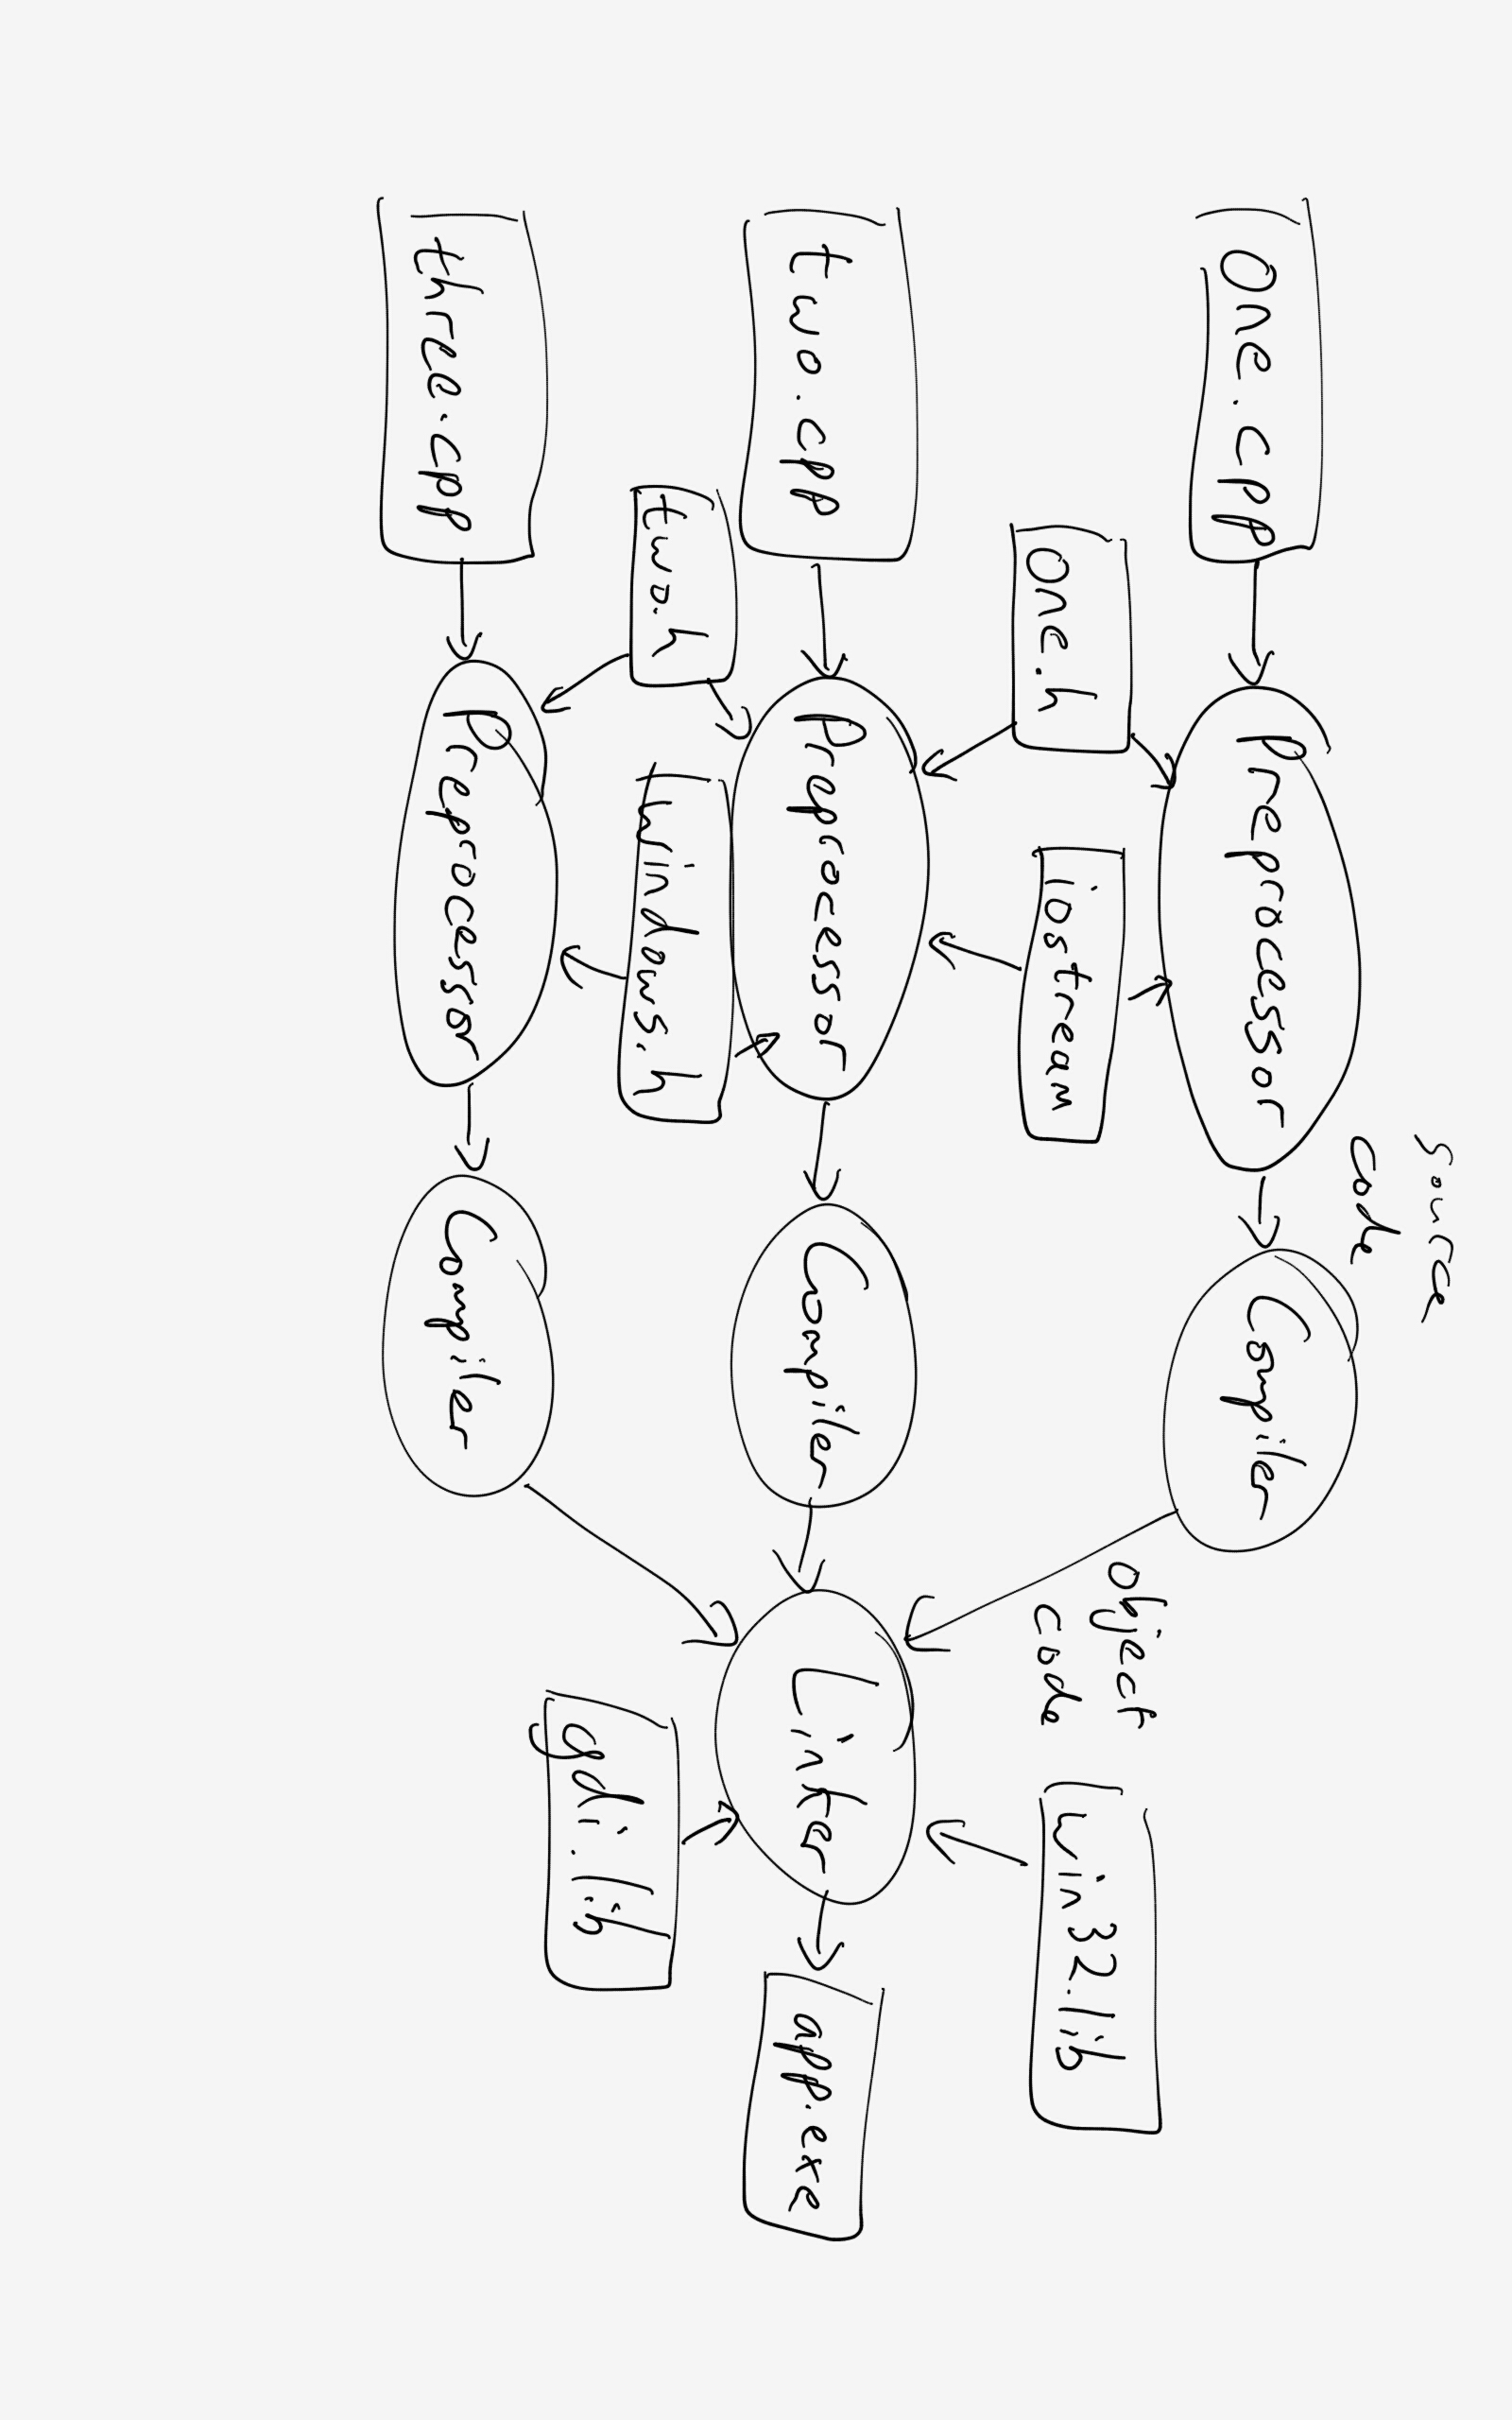
\includegraphics[height=\textwidth,angle=90]{compiler_sketch}
%\end{frame}

\end{document}
